\documentclass{article}\usepackage[]{graphicx}\usepackage[]{xcolor}
% maxwidth is the original width if it is less than linewidth
% otherwise use linewidth (to make sure the graphics do not exceed the margin)
\makeatletter
\def\maxwidth{ %
  \ifdim\Gin@nat@width>\linewidth
    \linewidth
  \else
    \Gin@nat@width
  \fi
}
\makeatother

\definecolor{fgcolor}{rgb}{0.345, 0.345, 0.345}
\newcommand{\hlnum}[1]{\textcolor[rgb]{0.686,0.059,0.569}{#1}}%
\newcommand{\hlsng}[1]{\textcolor[rgb]{0.192,0.494,0.8}{#1}}%
\newcommand{\hlcom}[1]{\textcolor[rgb]{0.678,0.584,0.686}{\textit{#1}}}%
\newcommand{\hlopt}[1]{\textcolor[rgb]{0,0,0}{#1}}%
\newcommand{\hldef}[1]{\textcolor[rgb]{0.345,0.345,0.345}{#1}}%
\newcommand{\hlkwa}[1]{\textcolor[rgb]{0.161,0.373,0.58}{\textbf{#1}}}%
\newcommand{\hlkwb}[1]{\textcolor[rgb]{0.69,0.353,0.396}{#1}}%
\newcommand{\hlkwc}[1]{\textcolor[rgb]{0.333,0.667,0.333}{#1}}%
\newcommand{\hlkwd}[1]{\textcolor[rgb]{0.737,0.353,0.396}{\textbf{#1}}}%
\let\hlipl\hlkwb

\usepackage{framed}
\makeatletter
\newenvironment{kframe}{%
 \def\at@end@of@kframe{}%
 \ifinner\ifhmode%
  \def\at@end@of@kframe{\end{minipage}}%
  \begin{minipage}{\columnwidth}%
 \fi\fi%
 \def\FrameCommand##1{\hskip\@totalleftmargin \hskip-\fboxsep
 \colorbox{shadecolor}{##1}\hskip-\fboxsep
     % There is no \\@totalrightmargin, so:
     \hskip-\linewidth \hskip-\@totalleftmargin \hskip\columnwidth}%
 \MakeFramed {\advance\hsize-\width
   \@totalleftmargin\z@ \linewidth\hsize
   \@setminipage}}%
 {\par\unskip\endMakeFramed%
 \at@end@of@kframe}
\makeatother

\definecolor{shadecolor}{rgb}{.97, .97, .97}
\definecolor{messagecolor}{rgb}{0, 0, 0}
\definecolor{warningcolor}{rgb}{1, 0, 1}
\definecolor{errorcolor}{rgb}{1, 0, 0}
\newenvironment{knitrout}{}{} % an empty environment to be redefined in TeX

\usepackage{alltt}
\usepackage{amsmath} %This allows me to use the align functionality.
                     %If you find yourself trying to replicate
                     %something you found online, ensure you're
                     %loading the necessary packages!
\usepackage{amsfonts}%Math font
\usepackage{graphicx}%For including graphics
\usepackage{hyperref}%For Hyperlinks
\usepackage[shortlabels]{enumitem}% For enumerated lists with labels specified
                                  % We had to run tlmgr_install("enumitem") in R
\hypersetup{colorlinks = true,citecolor=black} %set citations to have black (not green) color
\usepackage{natbib}        %For the bibliography
\setlength{\bibsep}{0pt plus 0.3ex}
\bibliographystyle{apalike}%For the bibliography
\usepackage[margin=0.50in]{geometry}
\usepackage{float}
\usepackage{multicol}

\usepackage{hyperref}

%fix for figures
\usepackage{caption}
\newenvironment{Figure}
  {\par\medskip\noindent\minipage{\linewidth}}
  {\endminipage\par\medskip}
\IfFileExists{upquote.sty}{\usepackage{upquote}}{}
\begin{document}

\vspace{-1in}
\title{Lab 5 -- MATH 240 -- Computational Statistics}

\author{
  Avery Johnson \\
  Colgate University  \\
  Department of Mathematics  \\
  {\tt aqjohnson@colgate.edu}
}

\date{}

\maketitle

\begin{multicols}{2}
\begin{abstract}
This lab aims to determine which band contributed most to the song ``Allentown" by analyzing sound and lyric features across multiple datasets.
We compiled music analysis extracted using Essentia, along with Essentia model data, and integrated it with LIWC-based lyric analysis. Our methodology involved feature selection to identify distinguishing characteristics among three bands and summary visualizations to support our conclusions. Results indicate that Manchester Orchestra had the largest impact on sound, while the Front Bottoms had the largest lyrical impact.

\end{abstract}

\noindent \textbf{Keywords:} libraries; character objects; for() loops;  vectors/lists; tidyverse; and summarizing data

\section{Introduction}

In 2018, the Front Bottoms, Manchester Orchestra, and All Get Out collaborated on a track called ``Allentown." To determine which band contributed most to the song, a data-driven analysis was conducted on their previous tracks. This task utilized Essentia \citep{essentia}, an open-source tool for music analysis, to extract audio features from 181 tracks. Given the large dataset, we developed a batch file to automate the command-line extraction process, streamlining data collection. We then cleaned and integrated the three key data sets: Essentia Extractor data \citep{essentia}, which captures detailed spectrogram-based sound analysis, Essentia Model data \citep{essentiamodel}, and LIWC data \citep{liwc}, which analyzes lyrical content. Building on this foundation, Lab 5 focused on feature selection and analysis to summarize the data, and therefore conclude which band had the largest impact on ``Allentown."

\section{Methods}

\subsection{Task 1: Automating Data Extraction}
To automate the execution of Essentia for each audio track, we created a batch file that systematically processed all .WAV files. Using the \texttt{stringr} package in \texttt{R} \citep{stringr}, we extracted subdirectories for each album, identified and counted the .WAV files, and constructed the command line calls to execute the Essentia program for each track using a \texttt{for} loop. 

\columnbreak

\subsection{Task 2: Compiling and Cleaning Data}
To analyze musical contributions, we compiled extracted data into a consolidated data frame. This involved processesing JSON files, integrating Essentia extractor and model data, and incorporating LIWC lyric analysis. After extracting relevant audio features, we loaded and cleaned the data. This involved using the \texttt{rowMeans()} to average feature values across different extractors. The data was then merged into a single data frame using the \texttt{merge()} function. Finally, using \texttt{write.csv}, the final dataset was stored in training and testing sets for further analysis.

\subsection{Task 3: Summarizing and Analyzing Feature Ranges}
Building on previous labs, we examined feature distributions across the dataset to determine which characteristics best differentiated the bands. To identify distinguishing features, we analyzed the range of values for each feature and classified them as out of range, outlying, or within range based on the min, max, lower fence, and upper fence thresholds. Specifically, features where two bands were out of range while one band remained within range were considered strong indicators of influence. From an initial selection of 20 features, we identified four key lyrical features (from LIWC) and 4 sound features (from Essentia) that were most relevant. We compiled these features into summary tables using  \texttt{xtable} and generated violin and box plots using \texttt{ggplot2} to visually assess differences across bands. The red dashed lines in the plots represent the corresponding feature values for ``Allentown," allowing us to determine which band's characteristics aligned most closely with the song.

\section{Results}

\subsection{Task 1 Results}
The \texttt{R} script successfully identified album subdirectories and filtered .WAV files. It then generated batch commands for each track, which were saved in a text file named \texttt{batfile.txt}. These commands generated the Essentia program for each track, saving the corresponding output as JSON files. The process was automated, enabling batch processing for all audio tracks.

\columnbreak


\subsection{Task 2 Results}
Task 2 involved first processing the JSON output for a single track. The artist, album, and track name were obtained from the file name, and relevant audio features were successfully extracted. An example of extracting one of these features from this song is shown below.


\begin{table}[H]
    \centering
    \begin{tabular}{|l|l|}
        \hline
        \textbf{Feature} & \textbf{Value} \\
        \hline
        Artist & The Front Bottoms \\
        Album & Talon Of The Hawk \\
        Track & Au Revoir (Adios) \\
        Avg. Loudness & 0.5450 \\
        \hline
    \end{tabular}
    \caption{Extracted Audio Feature for ``Au Revoir (Adios)"}
    \label{tab:audio_features}
\end{table}

This process was scaled to the full dataset by extracting, cleaning, and merging the Essentia Extractor, Essentia Model, and LIWC data into a single dataframe called \texttt{merged\_df}, with 181 tracks and 140 features. Training data \texttt{trainingdata.csv} excluded ``Allentown," while testing data \texttt{testingdata.csv} contained only ``Allentown." These successfully written CSV files will help determine which band contributed most to the song. 


\subsection{Task 3 Results}
Our analysis for task 3 involved identifying features where only one band remained within range. We specifically focused on four lyrical and four audio-based features. This analysis for the sound data can be seen in Table 2 below.



% latex table generated in R 4.4.2 by xtable 1.8-4 package
% Mon Feb 24 22:50:52 2025
\begin{table}[H]
\centering
\begingroup\small
\begin{tabular}{lll}
  \hline
artist & description & feature \\ 
  \hline
All Get Out & Out of Range & spectral\_rolloff \\ 
  Manchester Orchestra & Within Range & spectral\_rolloff \\ 
  The Front Bottoms & Out of Range & spectral\_rolloff \\ 
  All Get Out & Outlying & dissonance \\ 
  Manchester Orchestra & Within Range & dissonance \\ 
  The Front Bottoms & Out of Range & dissonance \\ 
  All Get Out & Outlying & average\_loudness \\ 
  Manchester Orchestra & Within Range & average\_loudness \\ 
  The Front Bottoms & Outlying & average\_loudness \\ 
  All Get Out & Outlying & chords\_strength \\ 
  Manchester Orchestra & Within Range & chords\_strength \\ 
  The Front Bottoms & Out of Range & chords\_strength \\ 
   \hline
\end{tabular}
\endgroup
\caption{Summary of Features Identifying Influencing Band} 
\end{table}

The full set of feature comparisons for both sound and lyrical features, along with the min, max, and fence values, are in the Appendix. Violin plots were created to show the range of values for each band, with red dashed lines representing the feature values for ``Allentown." We analyzed four lyrical features (positivewords, OtherP, Perception, and conj) and four sound features (spectral\_rolloff, average\_loudness, chords\_strength, and dissonance). Figure 1 shows the violin plot for average\_loudness, where ``Allentown" aligns most closely with the Manchester Orchestra, suggesting they contributed most to the track's loudness. Similar analyses for the lyrical and other sound features can be found in Figures 2 and 3 in the Appendix. The results indicate that the Front Bottoms most influenced the lyrics, while the Manchester Orchestra had the greatest impact on the sound.

\begin{knitrout}\scriptsize
\definecolor{shadecolor}{rgb}{0.969, 0.969, 0.969}\color{fgcolor}
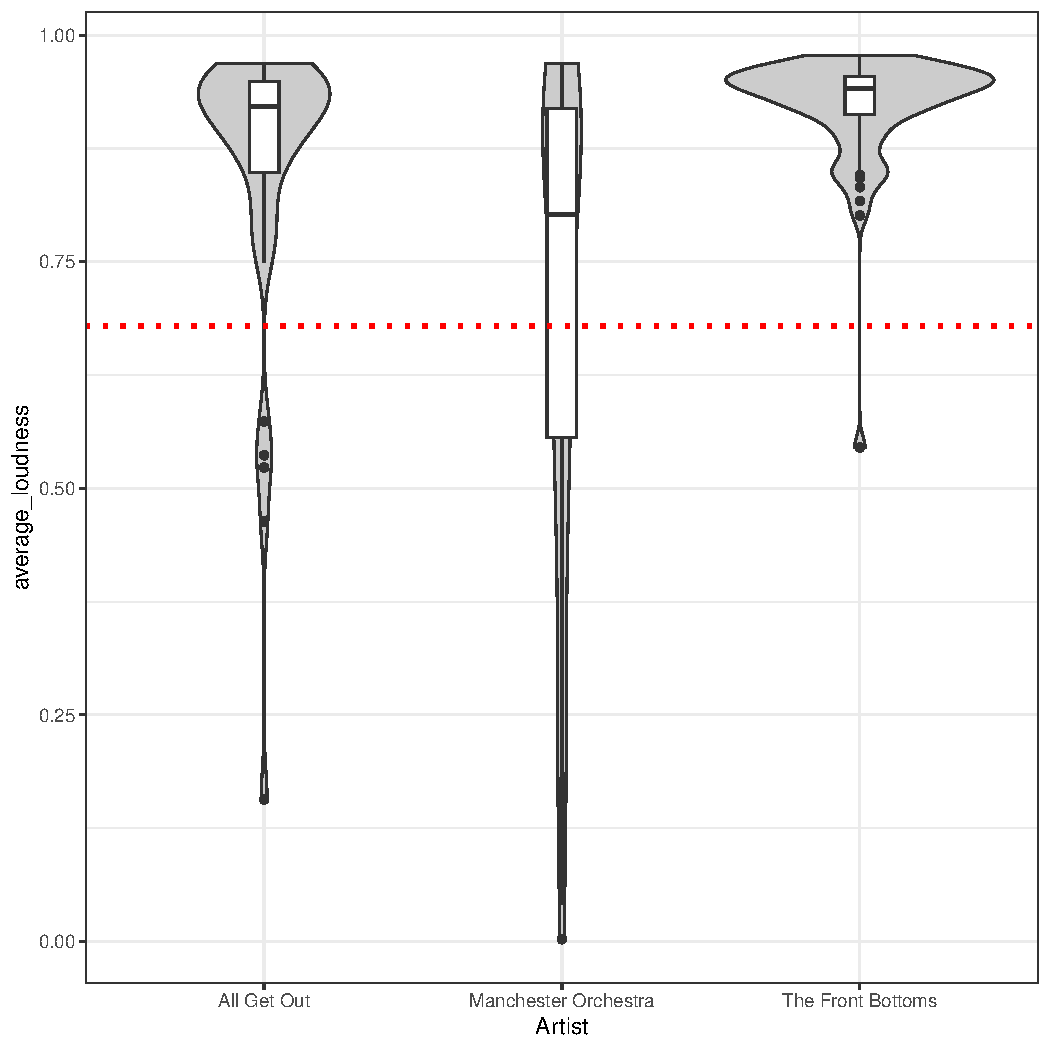
\includegraphics[width=\maxwidth]{figure/plot1-1} 
\end{knitrout}

\begin{figure}[H]
\begin{center}

\caption{Average Loudness by Band}
\label{averageloudness} %we can now reference plot1
\end{center}
\end{figure}

\section{Discussion}
This analysis identified key musical and lyrical features suggesting which band contributed most to ``Allentown." Lab 2 demonstrated the process of building a batch file and processing a single JSON output, while Lab 3 showed the scalability of this methodology by analyzing the full dataset. Statistical analysis revelaed that Manchester Orchestra most influenced the sound of ``Allentown," with features consistently in range, while the Front Bottoms impacted the lyrics, as their features aligned with ``Allentown" and others did not. The compiled summary and visual representations proviide a quantitative basis for these conclusions. However, the way the data were summarized is specific to our approach. Alternative methods for feature selections could potentially yield different results. This highlights the importance of methodological choices and suggests that future studies could explore other analytical techniques for comparison.

%%%%%%%%%%%%%%%%%%%%%%%%%%%%%%%%%%%%%%%%%%%%%%%%%%%%%%%%%%%%%%%%%%%%%%%%%%%%%%%%
% Bibliography
%%%%%%%%%%%%%%%%%%%%%%%%%%%%%%%%%%%%%%%%%%%%%%%%%%%%%%%%%%%%%%%%%%%%%%%%%%%%%%%%
\vspace{2em}

\begin{tiny}
\bibliography{bib}
\end{tiny}
\end{multicols}

%%%%%%%%%%%%%%%%%%%%%%%%%%%%%%%%%%%%%%%%%%%%%%%%%%%%%%%%%%%%%%%%%%%%%%%%%%%%%%%%
% Appendix
%%%%%%%%%%%%%%%%%%%%%%%%%%%%%%%%%%%%%%%%%%%%%%%%%%%%%%%%%%%%%%%%%%%%%%%%%%%%%%%%
\newpage
\onecolumn
\section{Appendix}

\begin{table}[ht]
\centering
\begin{tabular}{rlrrrrll}
  \hline
 & artist & min & max & LF & UF & description & feature \\ 
  \hline
1 & All Get Out & 935.91 & 2520.04 & 701.91 & 2767.30 & Out of Range & spectral\_rolloff \\ 
  2 & Manchester Orchestra & 518.87 & 2566.67 & 151.27 & 2083.17 & Within Range & spectral\_rolloff \\ 
  3 & The Front Bottoms & 927.04 & 3190.29 & 740.58 & 2421.46 & Out of Range & spectral\_rolloff \\ 
  4 & All Get Out & 0.40 & 0.48 & 0.44 & 0.50 & Outlying & dissonance \\ 
  5 & Manchester Orchestra & 0.37 & 0.48 & 0.36 & 0.53 & Within Range & dissonance \\ 
  6 & The Front Bottoms & 0.43 & 0.48 & 0.44 & 0.49 & Out of Range & dissonance \\ 
  7 & All Get Out & 0.16 & 0.97 & 0.70 & 1.10 & Outlying & average\_loudness \\ 
  8 & Manchester Orchestra & 0.00 & 0.97 & 0.01 & 1.46 & Within Range & average\_loudness \\ 
  9 & The Front Bottoms & 0.55 & 0.98 & 0.85 & 1.02 & Outlying & average\_loudness \\ 
  10 & All Get Out & 0.47 & 0.59 & 0.47 & 0.58 & Outlying & chords\_strength \\ 
  11 & Manchester Orchestra & 0.48 & 0.62 & 0.45 & 0.63 & Within Range & chords\_strength \\ 
  12 & The Front Bottoms & 0.48 & 0.57 & 0.46 & 0.58 & Out of Range & chords\_strength \\ 
  13 & All Get Out & 0.91 & 10.68 & -0.51 & 9.76 & Out of Range & conj \\ 
  14 & Manchester Orchestra & 0.00 & 14.43 & 0.74 & 10.98 & Outlying & conj \\ 
  15 & The Front Bottoms & 0.00 & 12.31 & -1.17 & 13.90 & Within Range & conj \\ 
  16 & All Get Out & 4.67 & 20.89 & 4.14 & 18.91 & Out of Range & Perception \\ 
  17 & Manchester Orchestra & 0.00 & 28.37 & -1.06 & 23.87 & Within Range & Perception \\ 
  18 & The Front Bottoms & 4.27 & 22.56 & 3.74 & 19.66 & Out of Range & Perception \\ 
  19 & All Get Out & 0.00 & 14.42 & -1.50 & 2.50 & Outlying & OtherP \\ 
  20 & Manchester Orchestra & 0.00 & 7.69 & -1.64 & 2.73 & Outlying & OtherP \\ 
  21 & The Front Bottoms & 0.00 & 12.50 & -3.48 & 7.20 & Within Range & OtherP \\ 
  22 & All Get Out & 2.00 & 58.00 & -1.50 & 18.50 & Outlying & positivewords \\ 
  23 & Manchester Orchestra & 0.00 & 27.00 & -3.00 & 13.00 & Outlying & positivewords \\ 
  24 & The Front Bottoms & 1.00 & 34.00 & -14.50 & 37.50 & Within Range & positivewords \\ 
   \hline
\end{tabular}
\caption{Full Summary of Key Features Identifying the Influencing Band} 
\end{table}

\begin{figure}[H]
\begin{center}
  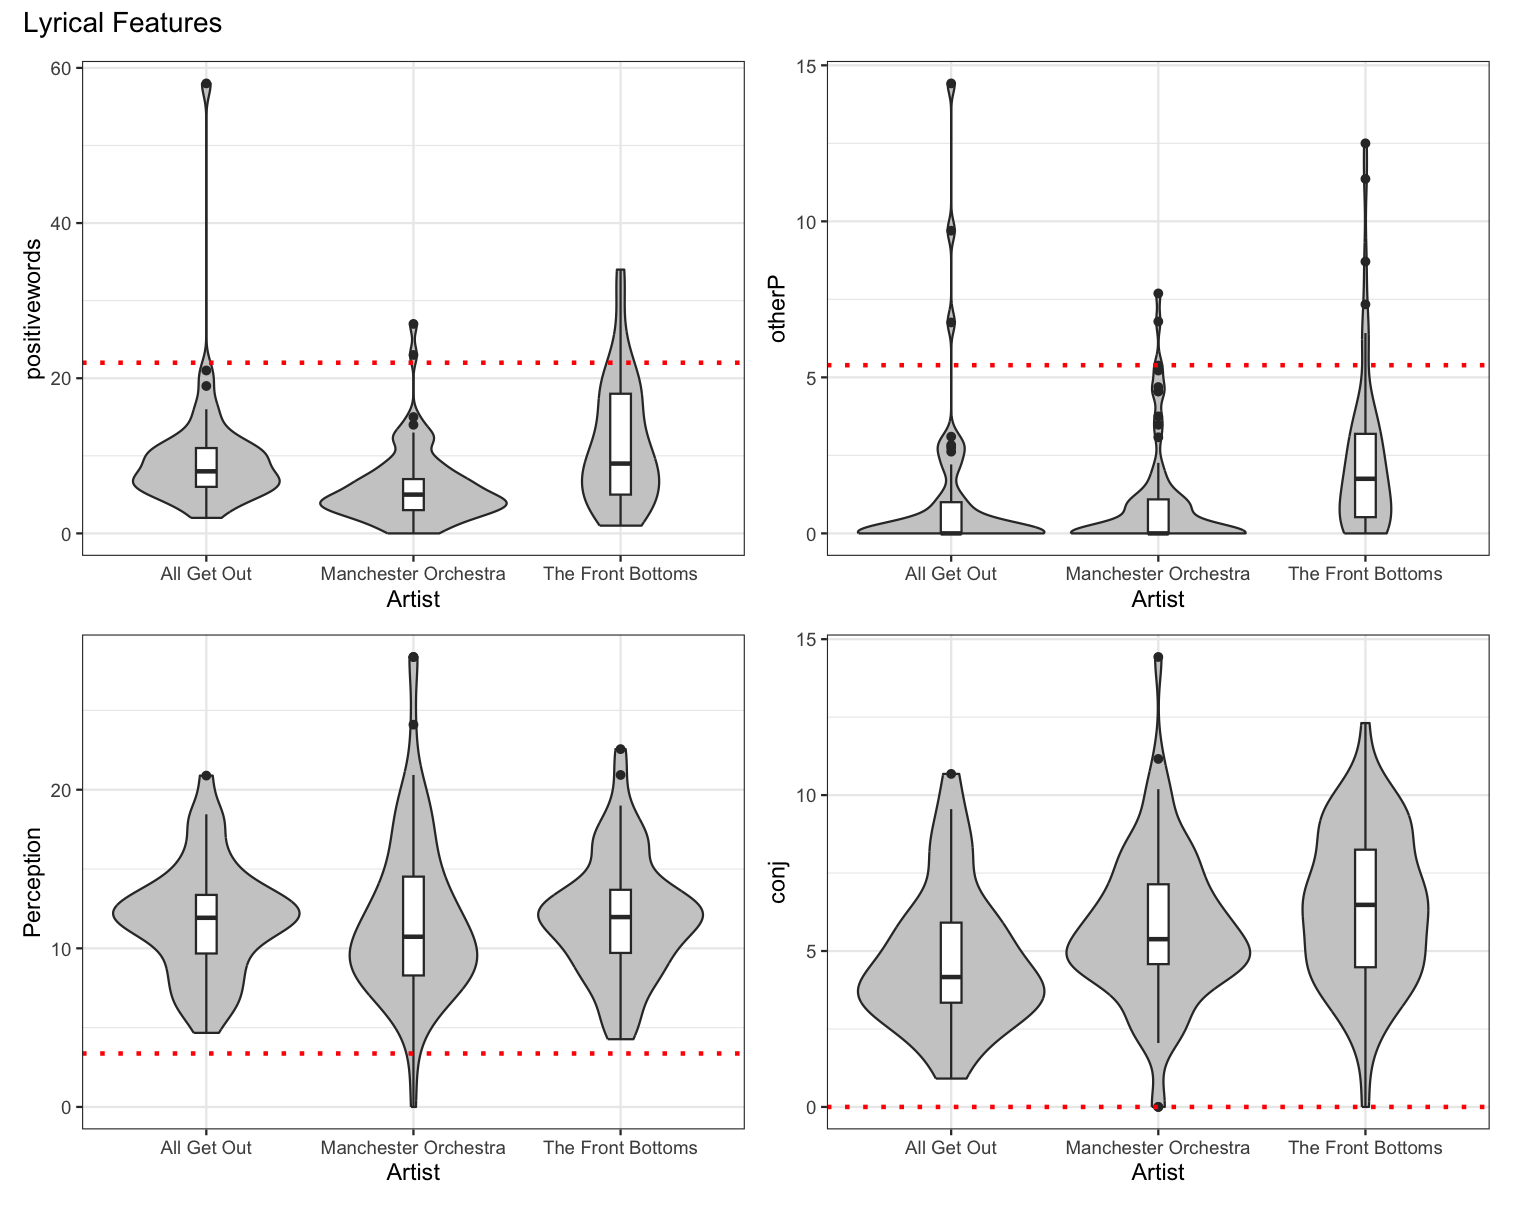
\includegraphics[width=\textwidth]{LyricFeaturesPlot.png}
  \caption{Lyrical Features}
  \label{lyricallarge}
\end{center}
\end{figure}

\begin{figure}[H]
\begin{center}
  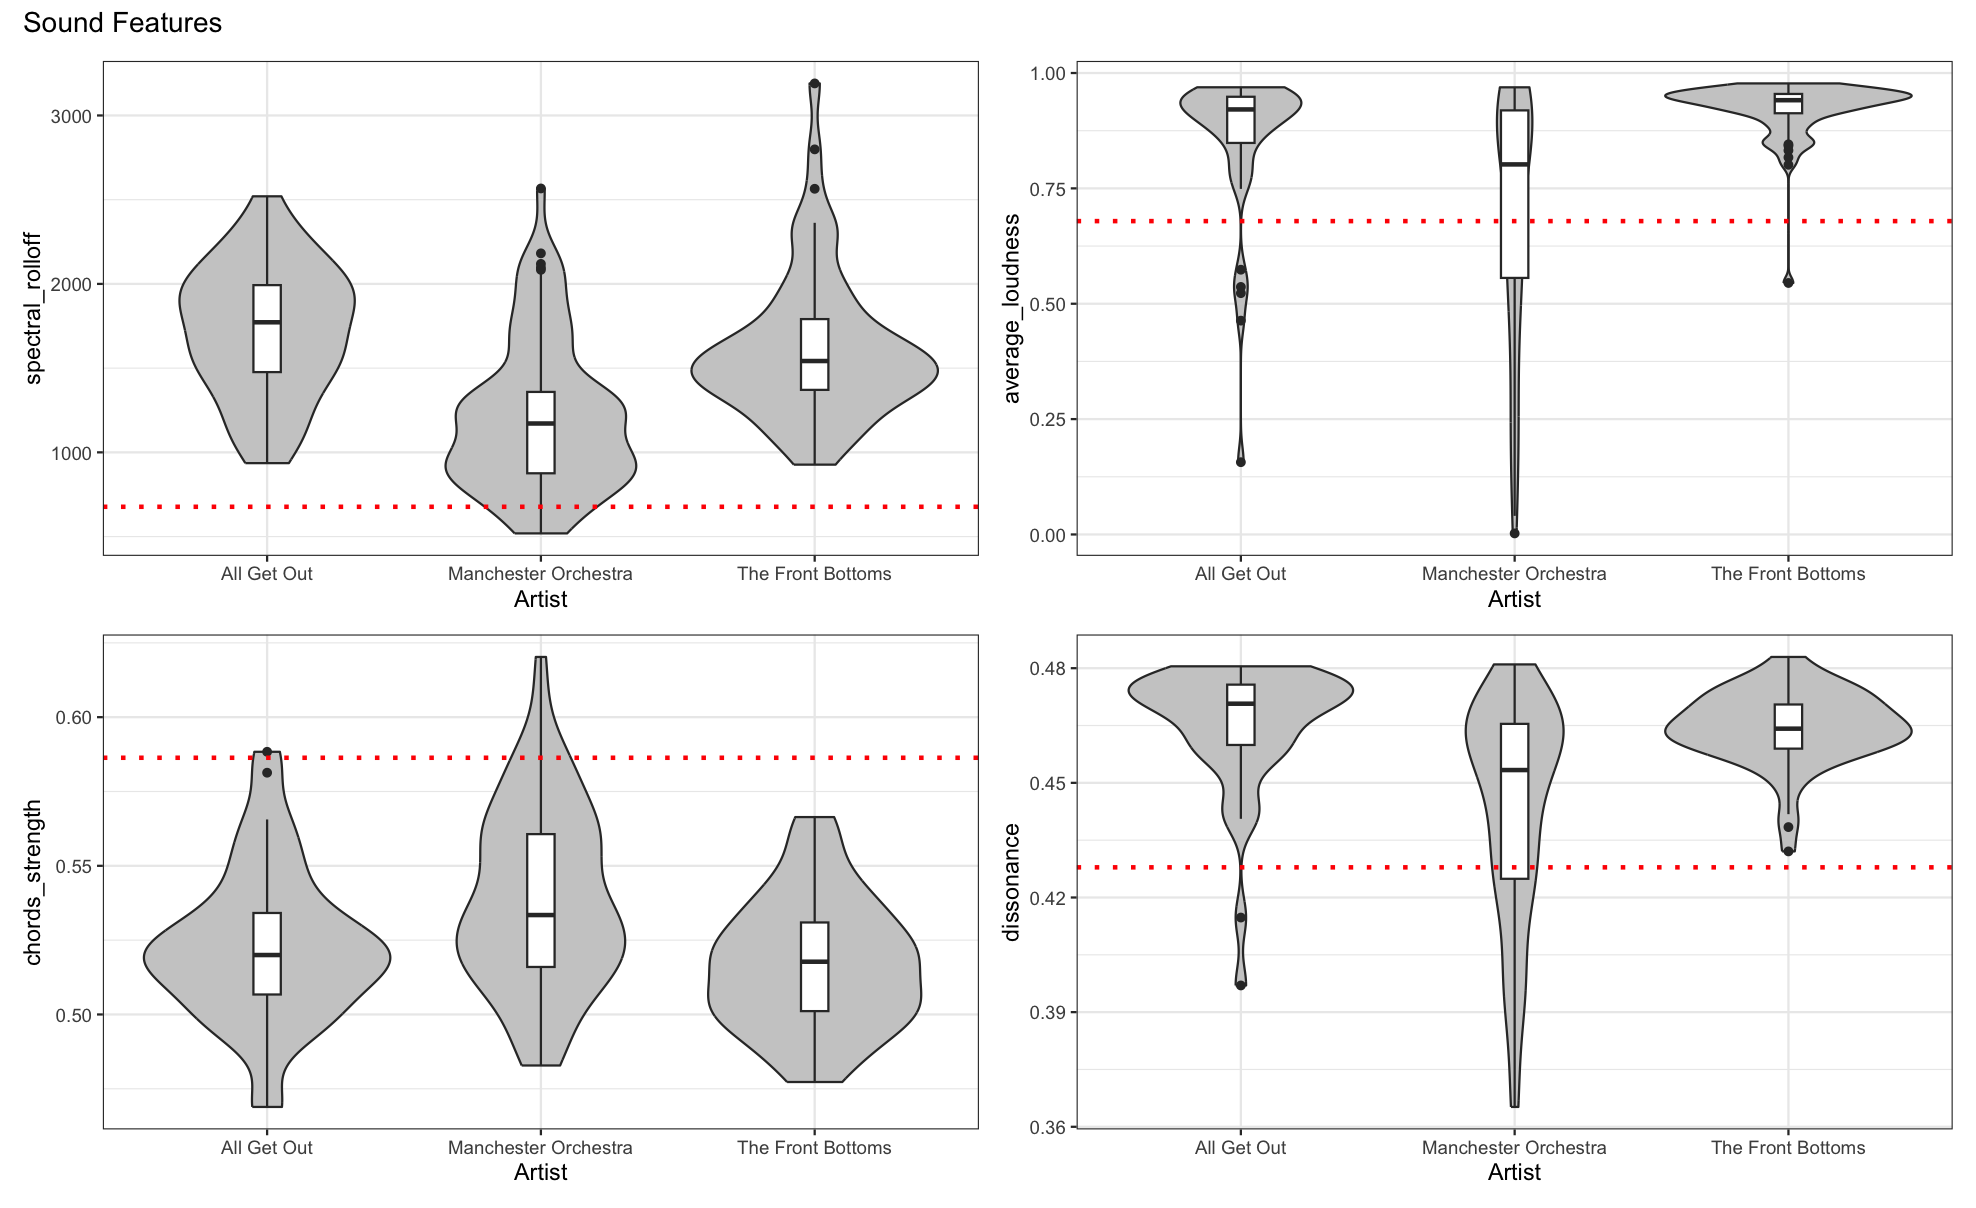
\includegraphics[width=\textwidth]{SoundFeaturesPlot.png}
  \caption{Sound Features}
  \label{soundlarge}
\end{center}
\end{figure}


\end{document}
